\documentclass[9pt,twocolumn,twoside,lineno]{pnas-new}
\usepackage{multirow} %connecting columns in tables
\usepackage{multicol}
% Use the lineno option to display guide line numbers if required.
% Note that the use of elements such as single-column equations
% may affect the guide line number alignment. 

\templatetype{pnasresearcharticle} % Choose template 
% {pnasresearcharticle} = Template for a two-column research article
% {pnasmathematics} = Template for a one-column mathematics article
% {pnasinvited} = Template for a PNAS invited submission

\title{Optimal control in the face of evolving resistance is an economic problem not a biological one.}

% Use letters for affiliations, numbers to show equal authorship (if applicable) and to indicate the corresponding author

\author[a,1]{Shaun R. Coutts}
\author[a]{Helen L. Hicks} 
\author[b]{Alexa Varah}
\author[c]{Kwadjo Ahodo}
\author[a]{Rob Freckleton}
\author[a]{Dylan Z. Childs}

\affil[a]{Animal and Plant Sciences, University of Sheffield, Sheffield S10 2TN, UK}
\affil[b]{Zoological Society of London, London NW1 4RY, UK}
\affil[c]{Kwadjo What should I put down here}

% Please give the surname of the lead author for the running footer
\leadauthor{Coutts} 

% Please add here a significance statement to explain the relevance of your work
\significancestatement{Integrated pest management (IPM) applies chemical and non-chemical control methods to pest populations to manage evolved resistance. However, we have a poor understanding of when different IPM strategies are incentivised. We find IPM strategies with the highest economic returns in an arable cropping system where high levels of herbicide resistance has evolved repeatedly. The best IPM strategies were dependent crop yields, yield loss caused by the weed, land tenure and levels of herbicide resistance. With the exception of herbicide resistance, all these factors are economic in nature. Knowing which IPM strategy to apply where will require, at a minimum, knowing the yield loss function for the major weeds of a farm, an economic problem rather than biological one.}

% Please include corresponding author, author contribution and author declaration information
\authorcontributions{SRC conceived the idea did the modelling and wrote the initial draft. HLH Collected field data for yield functions and aided in their interpretation. KA advised on economic cost modelling. All authors contributed to refining the focus and writing final manuscript.}
\authordeclaration{No conflicts of interest.}
\correspondingauthor{\textsuperscript{1}To whom correspondence should be addressed. E-mail: shaun.coutts\@gmail.com}

% Keywords are not mandatory, but authors are strongly encouraged to provide them. If provided, please include two to five keywords, separated by the pipe symbol, e.g:
\keywords{Integrated Pest Management $|$ herbicide resistance $|$ \textit{Alopecurus myosuroides} $|$ combinatorial optimisation} 

\begin{abstract}
Evolved resistance to xenobiotics (i.e. antibiotics, herbicides, pesticides, fungicides) is a global threat to public health and food security. In agricultural systems non-chemical control methods can be combined with xenobiotics (Integrated Pest Management; IPM) to prolong the useful life of compounds and manage pest populations after resistance has evolved. We find IPM strategies with the highest economic returns for an arable cropping system, and perform a global sensitivity analysis to find the factors that shape those strategies. The key uncertainties we find are economic in nature, and farmers have an economic incentive to be responsive to changes in weed the shape of the yield loss function. Doing so will require estimating, at a minimum, what yields would be in the absence of the pest, and how yields change with increasing pest density, with enough detail to say how much control (if any) is justified.            
\end{abstract}

\dates{This manuscript was compiled on \today}
\doi{\url{www.pnas.org/cgi/doi/10.1073/pnas.XXXXXXXXXX}}

\begin{document}

% Optional adjustment to line up main text (after abstract) of first page with line numbers, when using both lineno and twocolumn options.
% You should only change this length when you've finalised the article contents.
\verticaladjustment{-2pt}

\maketitle
\thispagestyle{firststyle}
\ifthenelse{\boolean{shortarticle}}{\ifthenelse{\boolean{singlecolumn}}{\abscontentformatted}{\abscontent}}{}

%Introduction
\dropcap{C}ontrolling populations in the face evolving resistance to xenobiotics (i.e. antibiotics, herbicides, pesticides, fungicides) is one of the biggest challenges facing public health \citep{Laxm2016, Willy2017}, and food security \citep{Denh1992, Palu2001, Hick2018}. Evolved resistance also costs billions of dollars globally \citep{Livi2016, Ches2018, Hick2018}. While there have been some successes in combating resistance in public health \citep{REX2013}, resistance is still a major problem in health care \citep{Willy2017} and there has been little success in other contexts, such as food production.

Current strategies to manage resistance focus on delaying the initial evolution of resistance by reducing the population (reducing the potential for \textit{de nova} resistance mutations), and killing any resistant mutants by using a second compound \citep{Denh1992, REX2013}. Multiple compounds are either stacked (used at the same time) or cycled in sequence. While these strategies can be effective in delaying the initial evolution of resistance they may be counter-productive if xenobiotic resistance is already present, which is true of important pests in food production systems \citep{Denh1992, Hick2018} and threats to human health \citep{Willy2017}. Strategies like stacking and cycling involve the continuous (and even increased) use of xenobiotics, which can help drive existing resistance through an entire population \citep{Denh1992, Hick2018}.

In agricultural systems chemical control can be used in combination with non-chemical control such as crop rotation, cultivation and spot control (e.g. hand-weeding), known as integrated pest management (IPM). IPM can be used both pro-actively to delay the evolution of resistance, and reactively to control pest populations as chemical control becomes less effective. While the concept of IPM is well established \citep{Bott1979}, finding good IPM strategies is challenging \citep{Dana2014, Chal2015}. Management tools need to be used in the correct combination and sequence to be most effective. This results in a very large number of potential IPM strategies (i.e. different combinations and sequences), even when considering only a handful of management tools and short time horizons \citep{Chal2015}. As a result there have been few attempts to rigorously search for good IPM strategies (see \citealp{Chal2015} for an exception). More commonly optimal strategies have looked for the best allocation between a few management options \citep{EpanN2010, Meis2016, Okum2016, Buyu2017}, and none have been developed where resistance could evolve to one of the primary management tools. These are important omissions for food production systems where resistance to xenobiotics has evolved numerous times \citep{Denh1992, Palu2001} and multiple non-chemical control options are available that can used in combination to deliver cost effective control \citep{Chal2015}.      

Little is known about how robust good IPM strategies are to changes in factors such as crop yield and pest population dynamics \citep{EpanN2010}. However, previous work on the optimal control of invasive populations has found general factors that shape optimal decisions. Biologically, a population's ability to escape density dependence shifts optimal control to younger age classes \citep{Pich2012}. The degree to which eradicated regions can be re-invaded also influences the optimal control strategies \citep{Janu2011, EpaN2012}, but the exact strategy depends on the way suitable habitats are connected \citep{Chads2011}. Economic factors tend to be at least as important as biological ones in shaping the optimal control strategy \citep{EpanN2010}. In particular the relationship between the density of an invasive species and the damage it does has been found to be crucial \citep{Yoko2009}. The way that future returns are valued also strongly influences the optimal control strategy; when more value is placed on future versus present returns more intensive control is favoured \citep{EpanN2010}.

We apply a genetic algorithm to a population model of an important weed of wheat in Europe (\textit{Alopecurus myosuroides}), where resistance to two herbicides can evolve. [ALEXA: sentence or two here + REF on just how damaging BG is]. To allow IPM strategies we also include crop rotation, cultivation and spot control as management options. We use global sensitivity analysis to determine the minimum information required to create a field scale IPM strategy that maximizes economic return and the impact of those strategies on herbicide resistance and economic gross margin.    

\section*{Results and Discussion}
Parameters defining the yield loss function (see Table \ref{tab:pars}) had the most influence on shaping incentivized IPM strategies. We used a linear yield loss function to relate density of \textit{A. myosuroides} to winter wheat yields, fit to data from 10 fields (Appendix 1). The intercept ($Y_0$) and slope of the yield function ($Y_D$) were two of the most important parameters (Fig. \ref{fig:rel_inf}). Another set of parameters that control how large the seed bank can become ($f_m$, $f_d$ and $\phi_b$) were also important. The potential size of the seed bank scales the x-axis of the yield function. Although yield functions have been estimated for major weeds \citep{Cous1985, Doyl1986, Swin1994}, there is evidence that yield functions vary substantially between fields \citep{Swin1994, Hick2018}, and little attention has been paid this variation and understanding its causes.
 \begin{figure}
	\centering
	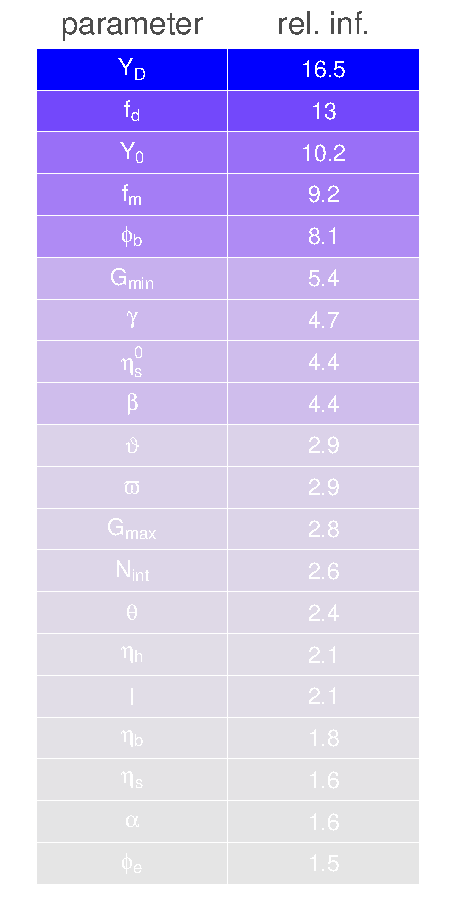
\includegraphics[height=80mm]{rel_inf_mean.pdf}
	\caption{Relative influence (relative reduction in squared error; \citealp{Mill2016}) of each parameter, averaged across dimensions of the solution space (Appendix 2). Values are scaled 0 to 100, with higher values indicating parameters with more influence on the structure of incentivized IPM strategies. See Table \ref{tab:pars} for an explanation of parameters.}
	\label{fig:rel_inf} 
\end{figure}

While the shape of the yield function is important, it may not be necessary to know it in great detail to find IPM strategies with high gross margin. When the yield of winter wheat with no \textit{A. myosuroides} ($Y_0$) was low, management intensity was lower and relied on crop rotation and tactical use of herbicide (Fig. \ref{fig:Y0_YD}, '$Y_0$ low'). The strategy changed little when slope of the yield function ($Y_D$) increased. Although, more herbicide was used when the value of $Y_D$ increased from a very low value to a higher value (1\% to 12\% losses at high densities of \textit{A. myosuroides}; Fig. \ref{fig:Y0_YD}g,e). When $Y_0$ was high, $Y_D$ showed two thresholds where IPM strategy changed. When $Y_D$ was very low the best strategy was to do noting and live with high populations of \textit{A. myosuroides} (Fig. \ref{fig:Y0_YD}h), since yield losses were never high enough to justify expenditure on control. Increasing $Y_D$ slightly meant some herbicide use and cultivation to rotate the seed bank became advantageous (Fig. \ref{fig:Y0_YD}f). Once $Y_D$ increased enough to justify intensive control, further increases did not change the IPM strategy (Fig. \ref{fig:Y0_YD}b,d). Thus, knowing how much management is justified by the yield loss function may only require having an estimate of the intercept ($Y_0$), and one or two thresholds values of $Y_D$, where a new IPM strategy becomes advantageous.
\begin{figure}
	\centering
	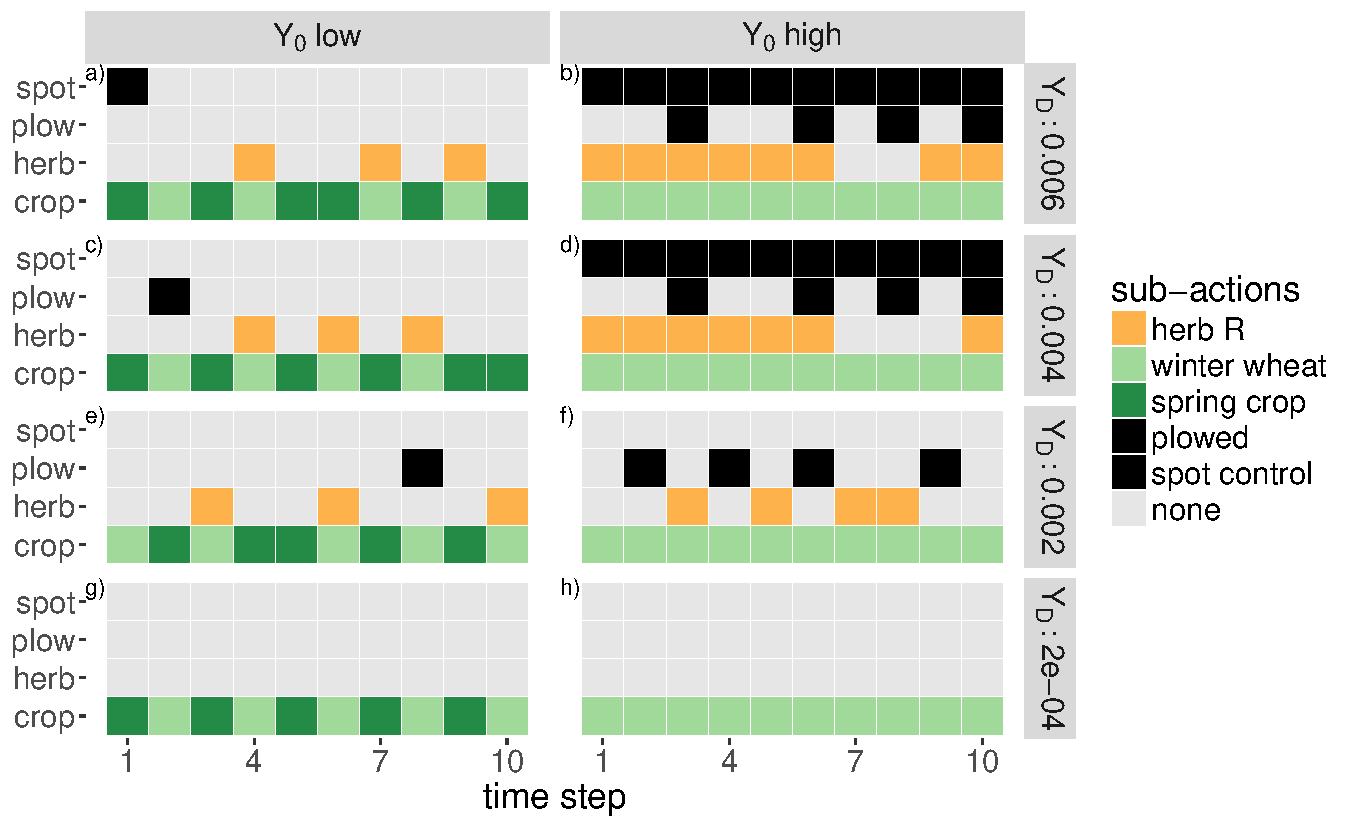
\includegraphics[width=1\linewidth]{MS_act_seq_YD_Y0.pdf}
	\caption{IPM strategies under high (\pounds 1668$\cdot$ha$^{-1}$) and low (\pounds 986$\cdot$ha$^{-1}$) values of $Y_0$ (yield of winter wheat with no \textit{A. myosuroides}), under increasing values (rows) of $Y_D$ (in \pounds$\cdot$plant$^{-1}\cdot$ha$^{-1}$). At the lower limit of $Y_D$ very high \textit{A. myosuroides} densities result in a 1\% yield loss under the high $Y_0$ scenario, and the upper limit implies a yield loss of 35\% . There is initially one effective herbicide ($R_\text{int} = 0.0001$, $Q_\text{int} = 0.9$).}
	\label{fig:Y0_YD} 
\end{figure}

Supporting previous work \citep{EpanN2010} we found higher values on future returns (larger values for $\gamma$) lead to more intensive IPM strategies. Intensive management to reduce the seed bank was only used when discount rates were high (Figure \ref{fig:dis_rate}). Recall that although we only show the first 10 years of IPM strategy, the discounted returns over 25 years are considered by the genetic algorithm. In agricultural systems land tenure have a crucial effect on how investments in weed control are valued. Those who own fields can benefit from long-term investments like weed control campaigns and soil conservation, whereas those who rent fields do not \citep{Wies1996, Fras2004}. 35\% of all agricultural land in England and Wales is under tenancy agreement \citep{CAAV2017}. This has important implications for the level of \textit{A. myosuroides} control managers are incentivised to provide, and thus its spread and the evolution of resistance.       
\begin{figure*}
	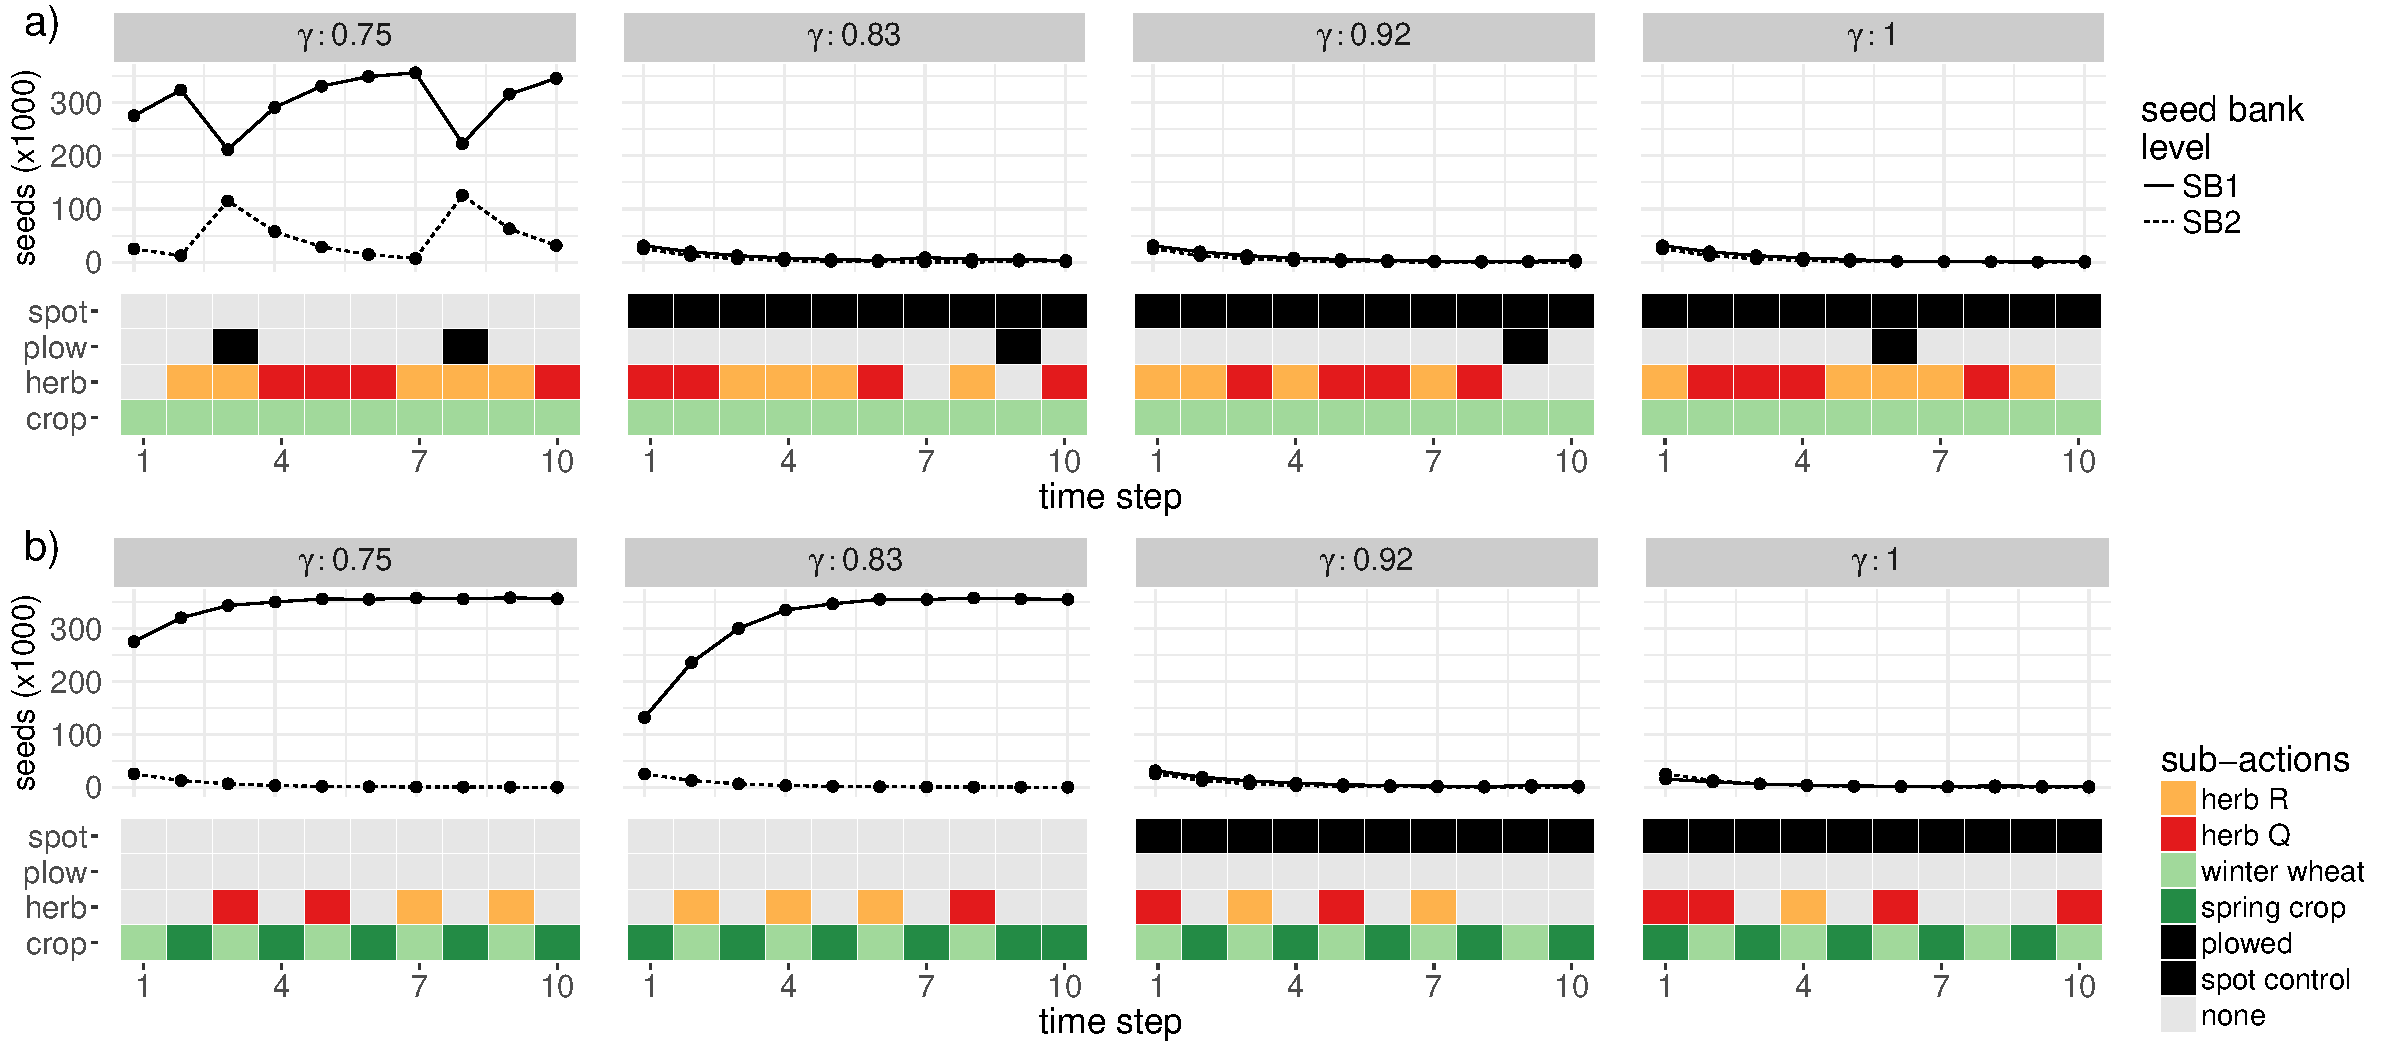
\includegraphics[width=178mm]{dis_rate_SB_strat.pdf}
	\caption{The effect of discount rate ($\gamma$) on the seed bank and IPM strategy (tile plots) when yields from winter wheat are high (a; \pounds 1668$\cdot$ha$^{-1}$) and low (b; \pounds 986$\cdot$ha$^{-1}$). In both cases the slope of the yield function ($Y_D$) is high (0.006\pounds$\cdot$plant$^{-1}\cdot$ha$^{-1}$). Initial resistance was low for both herbicides.}
	\label{fig:dis_rate} 
\end{figure*}

When both herbicides were effective the preference was to cycle between them, however even this did not prolong their continued use by much. Even when both $R$ and $Q$ started at frequencies of 1 in 20,000 alleles (Figure \ref{fig:int_res}a) continued herbicide use raised those frequencies to 1 in 50 within 10 time steps. This frequency provided enough variation for selection to rapidly act on (Figure \ref{fig:int_res}c). 

We present the best case that can be hoped for in reactive management, as we assume that herbicide resistance was conferred by target site mutations. This is why cycling was often favoured over stacking, as cycling prolonged the useful life of both herbicides since the application of each was spread out. However, there is growing evidence that non-target site resistance, which confers cross resistance, is widespread \citep{Hick2018}. If generalized, non-target site resistance mechanisms are present, the total amount of herbicide exposure predicts resistance level \citep{Hick2018}, and cycling will not help.

Even when initial frequencies of resistance to the remaining effective herbicide was low (1 in 200; Figure \ref{fig:int_res}c) initial continual use quickly drove the evolution of resistance to levels where herbicide use was greatly reduced after just five generations. As the initial frequency of resistance to the remaining effective herbicide ('herb Q' in this case) increased, even moderate herbicide use drove the rapid evolution of herbicide resistance. With an initial frequency of resistance alleles of 1 in 20 even three herbicide applications were enough to increase resistance to the point where applying both herbicides would result in 40\% survival (Figure \ref{fig:int_res}d). Once this situation was reached, gross margin was reduced by a quarter compared to returns with low resistance. 

This is in contrast to current management practice in this cropping system, where multiple herbicide applications a year are the norm, despite high levels of resistance \citep{Hick2018}. This disparity could arise from a number of contributing factors. Some managers may believe that even a little control (mortality of a few susceptible individuals) is better than no control and inaction is seen as the worst approach to weed management \citep{Wils2008}. In addition, IPM strategies are often seen as complex in comparison to routine application of chemicals, and having a steep learning curve \citep{Llew2006}. Resistance tends to be partial and build up slowly \citep{Moss2009, Hull2014}, so farmers may be victims of a shifting baseline, lowering their expectations of efficacy of weed control. There may be a belief that new herbicides will become available, despite no new modes of action being marketed for over 20 years \citep{Duke2012}. Thus, current strategies are viewed as a bridging strategy until a new product is found \citep{Hurl2016}. Finally, Our population model was deterministic, so IPM strategies could not be risk averse to variability in \textit{A. myosuroides} populations and economics factors like crop prices. Uncertainty in when herbicide resistance will emerge and the efficacy of non-chemical control can be a major impediment to adopting IPM \citep{Hurl2016}.     

\begin{figure*}[!ht]
	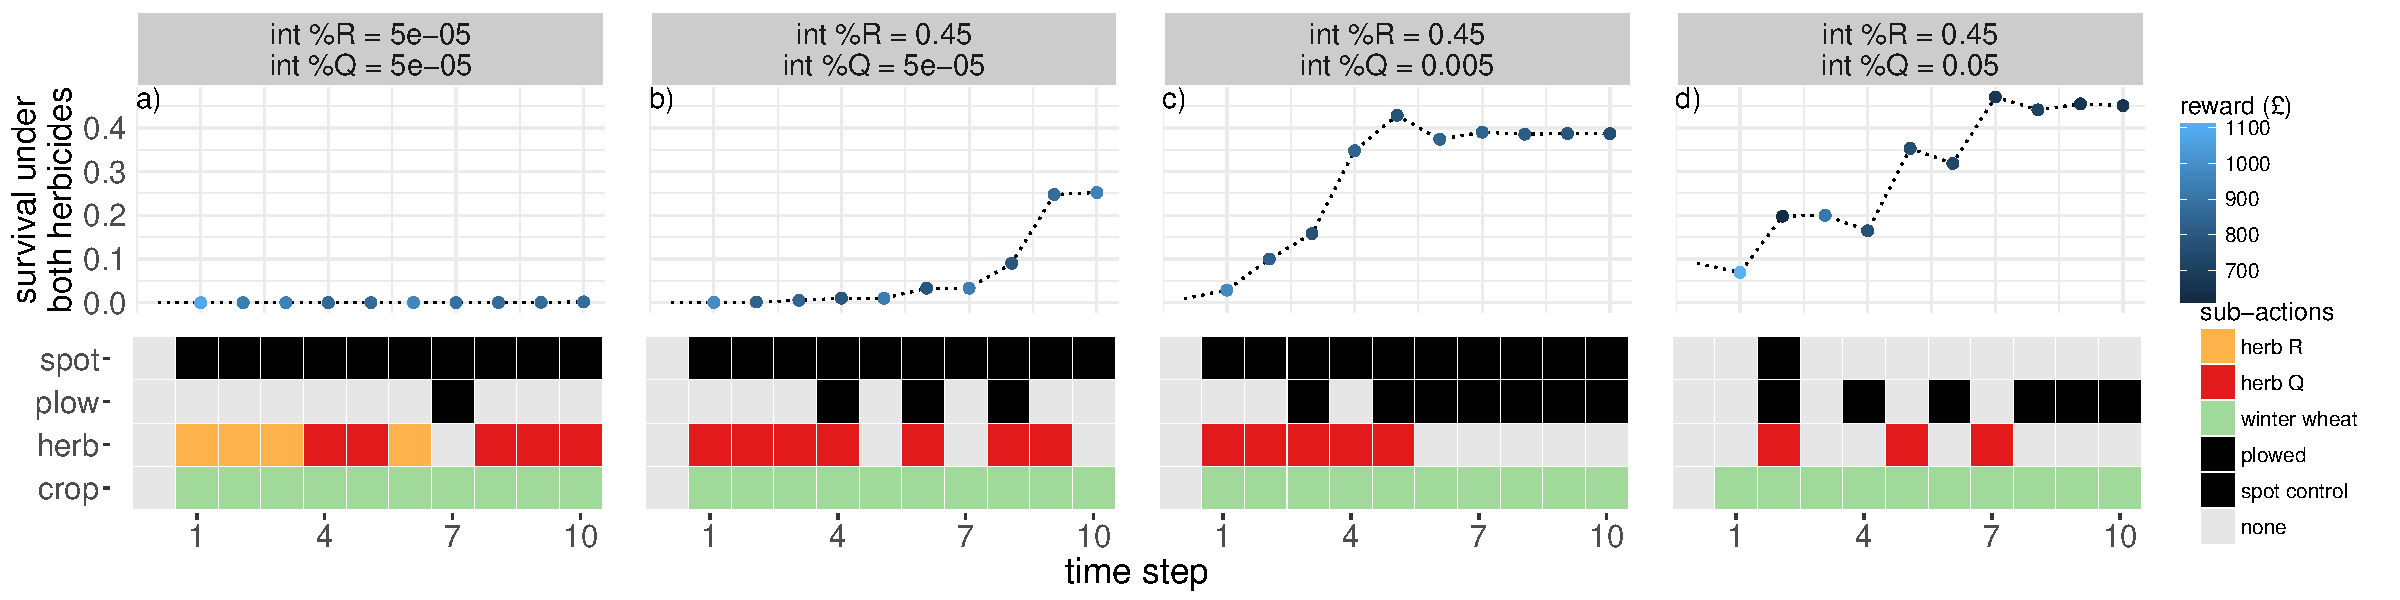
\includegraphics[width=178mm]{int_res_strat_resist.pdf}
	\caption{The effect of initial resistance on the selected IPM strategy (tile plots) and the evolution of herbicide resistance (\% survival to under both herbicides). Lighter coloured points indicate higher reward (gross margin) obtained in that time step. In this case $Y_0 = 1668$ (high winter wheat yield) and $Y_D = 0.0062$ (high yield penalty).}
	\label{fig:int_res} 
\end{figure*}

We assume that herbicide is the only action that drives the evolution of resistance. Any effective management tool will impose selection pressure, and so drive resistance to that tool. In reality, the spring cropping and spot control sub-actions make heavy use of glyphosate to control \textit{A. myosuroides}. Glyphosate resistance has evolved on many separate occasions in response to prolonged, heavy use \citep{Samm2014}. As glyphosate becomes a more important part of weed management \citep{Hick2018} resistance is likely. 

\section*{Conclusion}
Combating xenobiotic resistance is ultimately a problem of behaviour change, and thus how individuals are incentivized to act \citep{Hurl2016}. Our results show that farmers have an economic incentive to be responsive to changes in weed the shape of the yield loss function. Doing so will require estimating, at a minimum, what yields would be in the absence of the pest, and how yields change with increasing pest density, with enough detail to say how much control (if any) is justified.    

[ALEXA: would be nice to conclude with a nice summary statement on what a failure to be responsive will cost farmers, the economy as whole and the environment, are at least as much as we can say at this point. Also be a good place to flag your up coming work for any things that are still unresolved. If it is all unresolved that is an important message as well I think.] 

\subsection*{Data Archival}

PNAS must be able to archive the data essential to a published article. Where such archiving is not possible, deposition of data in public databases, such as GenBank, ArrayExpress, Protein Data Bank, Unidata, and others outlined in the Information for Authors, is acceptable.

\begin{table}%[tbhp]
\centering
\caption{Parameter descriptions}\label{tab:pars}	
\begin{tabular}{c p{6.5cm}}
Parameter & Description \\
\midrule
% table of parameters and ranges used
	\multicolumn{2}{l}{\textit{Population Model  see Appendix 3}}\\
	$\phi_e$ & germination probability \\ 
	$\phi_b$ & Probability a seed survives one year \\
	$s_0$ & Survival probability without herbicide \\
	$\theta$ & Proportion of \textit{A. myosuroides} population exposed to herbicide under sub-action $a_h$ = herb R, herb Q or both. plants may be missed spatially or temporally, or spraying may be affected by rain. \\       
	$s_h$ & Survival of susceptible \textit{A. myosuroides} exposed to herbicide ($a_h$). Herbicide assumed to be effective.\\
	$\alpha$ & Survival probability under the alternative crop ($a_k$ = alt), spring barley. \\
	$\beta$ & Survival under spot control (sub-action $a_s$), for example because plants are missed. \\
	$f_m$ & \multirow{2}{6.5cm}{\parbox[t]{6.5cm}{Seeds$\cdot$plant$^{-1}$ when density is 0 ($f_m$) and the effect of density on seed production ($f_d$) interact to determine maximum population size. Values chosen to keep the max population close to the maximum population seen in \citet{Quee2011} so yield is not extrapolated outside the observed range.}} \\
	$f_d$ & \\\\\\\\
	$I$ & The proportion of seed moved between seed bank levels by ploughing (sub-action $a_b$) \\ 
	\multicolumn{2}{l}{\textit{Reward function see Appendix 1}}\\
	$\gamma$ & discount rate on future returns. \\
	$Y_0$ & Yield in \pounds $\cdot ha^{-1}$ from winter wheat when \textit{A. myosuroides} is absent. \\
	$Y_D$ & reduction in yield caused by each \textit{A. myosuroides} (in \pounds$\cdot$plant$\cdot$ha$^{-1}$). \\
	$\vartheta$ & Yield of spring barley in \pounds$\cdot ha^{-1}$, an alternative crop commonly used to control \textit{A. myosuroides}. \\
	 $\varpi$ & Proportion of yield achieved if crop $a_k$ is repeated \\
	 $\eta_h$ & Cost of a single herbicide application in \pounds$\cdot$ha$^{-1}$. \\
	 $\eta_b$ & Cost of ploughing in \pounds$\cdot$ha$^{-1}$. \\
	 $\eta_s^0$ & Cost of spot control even when \textit{A. myosuroides} density is 0, in \pounds$\cdot$ha$^{-1}$. \\
	 $\eta_s$ & Increase in spot control cost for each \textit{A. myosuroides} in \pounds$\cdot$plant$^{-1}\cdot$ha$^{-1}$ \\
	 $\eta_k$ & Costs of crop $a_k$, in \pounds$\cdot$ha$^{-1}$, not associated with the other sub-actions targeted at \textit{A. myosuroides} control. \\ 
	\multicolumn{2}{l}{\textit{Initial Conditions}}\\
	$G_\text{min/max}$ & Initial allele frequency of mutants resistant to the herbicide with the lowest (min) and highest (max) population level resistance. \\
	$N_\text{int}$ & Initial number of seeds in each level of the seed bank \\
\bottomrule
\end{tabular}
\end{table}

\subsection*{Supporting Information (SI)}
\subsubsection*{Appendices}
Appendix 1: Reward Function\\
Appendix 2: Finding Which Initial Conditions and Model Parameters Lead to Which IPM Strategies\\
Appendix 3: Population Model\\
Appendix 4: Action Space\\
Appendix 5: Genetic Algorithm\\

%METHODS
\matmethods{We frame IPM as a combinatorial optimisation problem where the goal is to find a good combination of management tools, used in sequence. We use a genetic algorithm to solve this combinatorial problem \citep{Tayl2004GA, Carr2010}. Genetic algorithms cannot be checked to have found the globally optimal solution, as this would require already knowing the solution. However, genetic algorithms are efficient at weeding out comparatively poor solutions, so that over successive iterations the regions of the solution space being explored gets progressively better, resulting in a set of good (often near optimal) solutions.

Our goal is to find good IPM strategies in the face of rapidly evolving resistance, and how those strategies change in response to biological and management parameters. This problem has fours parts: i) A reward function that measures how good a given IPM strategy is based on how much that strategy cost and its effectiveness, we use net present economic value. ii) A population model that translates a given IPM strategy into a population, and thus a reward. iii) An algorithm that finds IPM strategies with higher rewards, the genetic algorithm. iv) Finally we need to relate changes in the best IPM strategy found to changes in initial conditions and model parameters. We use a meta-modelling global sensitivity analysis \citep{Cout2014} based on multi-variate boosted regression trees \citep{Mill2016}. 

\subsection*{Population model}
The population model links management actions to the response of the \textit{A. myosuroides} population, and thus wheat yields. The action $a_j$ is how the manager effects the population model, and thus the reward they get. Each action is a tuple of four sub-actions $a_j = \langle a_h, a_b, a_k, a_s \rangle$, see Appendix 4 for a description of the sub-actions and all eligible combinations of these sub-actions (i.e. the full actions space, $\mathbf{A}$). 

The processes included in the population model limit the scope of the IPM strategies found. We use a deterministic model, and so our IPM strategies can only deal with average expected population responses, ignoring demographic uncertainty, and environmental and market variability. Also, we only model herbicide resistance that is already present in the population because \textit{de nova} mutation is a fundamentally stochastic process. 

A commonly recommended \citep{REX2013} and applied \citep{Hick2018} strategy to combat resistance is to apply xenobiotics that impair different cellar pathways (i.e. modes of action), either sequentially (cycling) or concurrently (stacking). To allow this behaviour we use a discrete time, spatially implicit model, where two independent alleles ($R$ and $Q$), each confer target site resistance to a separate herbicide. The model must also be flexible enough to accommodate non-chemical control. We include a two level seed bank (to allow plowing to take seeds out of the germinating population) and model survival as a function of resistance, herbicide choice, crop choice and spot control (where the cost increases with \textit{A. myosuroides} density). The model tracks the number of seeds in each level of the seed bank in each of nine genotypes $G$, starting at the beginning of the growing season before any seeds have emerged. See Appendix 3 for a full description of the model and how each sub-action affects the population. 

\subsection*{Reward function}
The reward function measures how good an IPM strategy is, given a initial starting condition and parameter set that the model is run under. The reward function encodes the goals of a manager. We assume farmers are primarily driven by economic returns. The economic return consists of two parts, the income made from the crop and the costs of producing that crop. We assume that usual farm costs, such as buildings and machinery as constant from year to year, so we focus on gross margin, i.e. income - variable costs \citep[pp.~3--4]{Nix2016}. 

To explicitly link the above ground population to the reward function we define $N''(\mathbf{a}, n_0, t)$, the total above ground population after all control actions, at time $t$ given an initial population $n_0$ and a sequence of actions 
\begin{equation}
	\mathbf{a} = \{a_j^0, a_j^1, \cdots, a_j^T\}
\end{equation}	  
where $a_j^t$ is the action $a_j \in \mathbf{A}$ taken at time $t$ and $T$ is the time horizon over which management is run. We assume all returns after $T$ are ignored. The reward function is  
\begin{equation}
	R(\mathbf{a}, n_0) = \sum_{t=0}^T \gamma^t \Big( Y(N''(\mathbf{a}, n_0, t)) - C(a_j^t) \Big)
\end{equation}
where $R(\mathbf{a}, n_0)$ is the time discounted reward for action sequence $\mathbf{a}$ given starting population $n_0$, $\gamma \in [0, 1]$ is the discount rate. When $\gamma = 0$ only the reward in the first time step is considered, when $\gamma = 1$ returns in all future time steps up to $T$ are valued equally. $Y(N''(\mathbf{a}, n_0, t))$ is the income (in \pounds /ha) from the crop chosen at time $t$ given start stating $n_0$ and following action sequence $\mathbf{a}$. $C(a_j)$ is the cost of taking action $a_j$, and is composed of the cost of controlling \textit{A. myosuroides} and other costs that depend in the crop being grown ($a_k$).   

See Appendix 1 for the yield and cost models for each sub-action and parameter estimation.

\subsection*{Finding good IPM strategies} 
Our goal is to find good strategists to manage black grass in the face of evolving resistance, however it is not feasible to test every combination of management options over more than a handful of years. Genetic algorithms have been used to find good solutions to this class of problem \citep{Tayl2004GA, Carr2010}. The genetic algorithm starts with an randomly generated set of action sequences, these action sequences are then iteratively improved to find a set of action sequences with a high gross margin. Genetic algorithms rely on the fact that even though the number of possible action sequences is large, many perform very poorly. The genetic algorithm explores better performing regions of the solution space more intensely. While genetic algorithms are not guaranteed to find the optimal action sequence they will find a set of actions sequences that perform well, often close to the optimal solution.   

To find good action sequences we use a genetic algorithm with knock out tournament selection, where each action sequence in a set of 1000 actions sequences is randomly paired with another, and the action sequence with the highest $R(\mathbf{a}, n_0)$ survives to help generate new action sequences. We used pair mating between survivors and N-point cross-over to produce new action sequences. After new action sequences are created there is a process of random mutation where each $a_j^t$ is changed to another $a_j^t \in \mathbf{A}$ with probability $m = 0.03$. The algorithm used is given in Appendix 5.        

\subsection*{Finding which initial conditions and model parameters lead to which IPM strategies}
It is unlikely a given IPM strategy will perform well in all scenarios. To find the parameters and initial conditions ($n_0$) that shaped the IPM strategy with the highest reward, we extend the meta-modelling approach to global sensitivity analysis outlined in \citet{Cout2014}, to multivariate time series outputs (i.e. the sequences of the four sub actions). We: i) ran the genetic algorithm under 15000 different parameter sets and initial conditions, generated with Latin hyper-cube sampling (see Table S1 in Appendix 2 for upper and lower limits of each parameter), ii) used Longest Common Sub-Sequence \citep{Tooh2015} as a measure of distance between these action sequences, iii) projected the resulting distance matrix into an 8D solution space using non-metric multi-dimensional scaling (implemented in the 'ecodist' R package; \citealt{Gosl2007}), iv) predicted where each IPM solution sat in the solution space using multi-variate boosted regression tree \citep{Mill2016}, where the model parameters and initial conditions were predictors. See Appendix 2 for details.

It was this multi-variate boosted regression tree we interrogated to find which parameters and initial conditions were important for changing the best IPM strategy found--using relative influence and partial dependence plots \citep{Mill2016}.    

}

\showmatmethods % Display the Materials and Methods section

\acknow{We thank the Rothamstead Farmer Focus group for valuable insight on IPM strategies.}

\showacknow % Display the acknowledgments section

% \pnasbreak splits and balances the columns before the references.
% If you see unexpected formatting errors, try commenting out this line
% as it can run into problems with floats and footnotes on the final page.
%\pnasbreak

% Bibliography
\bibliography{/Users/shauncoutts/Dropbox/shauns_paper/referencing/refs} 

\end{document}